%%
%% Copyright 2007, 2008, 2009 Elsevier Ltd
%%
%% This file is part of the 'Elsarticle Bundle'.
%% ---------------------------------------------
%%
%% It may be distributed under the conditions of the LaTeX Project Public
%% License, either version 1.2 of this license or (at your option) any
%% later version.  The latest version of this license is in
%%    http://www.latex-project.org/lppl.txt
%% and version 1.2 or later is part of all distributions of LaTeX
%% version 1999/12/01 or later.
%%
%% This template has been modified by Philip Blakely for
%% local distribution to students on the MPhil for Scientific
%% Computing course run at the University of Cambridge.
%%

%% Template article for Elsevier's document class `elsarticle'
%% with numbered style bibliographic references
%% SP 2008/03/01
%%
%%
%%
%% $Id: elsarticle-template-num.tex 4 2009-10-24 08:22:58Z rishi $
%%
%%
\documentclass[final,3p,times,twocolumn]{elsarticle}

%% Use the option review to obtain double line spacing
%% \documentclass[preprint,review,12pt]{elsarticle}

%% Use the options 1p,twocolumn; 3p; 3p,twocolumn; 5p; or 5p,twocolumn
%% for a journal layout:
%% \documentclass[final,1p,times]{elsarticle}
%% \documentclass[final,1p,times,twocolumn]{elsarticle}
%% \documentclass[final,3p,times]{elsarticle}
%% \documentclass[final,3p,times,twocolumn]{elsarticle}
%% \documentclass[final,5p,times]{elsarticle}
%% \documentclass[final,5p,times,twocolumn]{elsarticle}

%% if you use PostScript figures in your article
%% use the graphics package for simple commands
%% \usepackage{graphics}
%% or use the graphicx package for more complicated commands
%% \usepackage{graphicx}
%% or use the epsfig package if you prefer to use the old commands
%% \usepackage{epsfig}

%% The amssymb package provides various useful mathematical symbols
\usepackage{amssymb}
%% The amsthm package provides extended theorem environments
%% \usepackage{amsthm}

%% The lineno packages adds line numbers. Start line numbering with
%% \begin{linenumbers}, end it with \end{linenumbers}. Or switch it on
%% for the whole article with \linenumbers after \end{frontmatter}.
%% \usepackage{lineno}

%% natbib.sty is loaded by default. However, natbib options can be
%% provided with \biboptions{...} command. Following options are
%% valid:

%%   round  -  round parentheses are used (default)
%%   square -  square brackets are used   [option]
%%   curly  -  curly braces are used      {option}
%%   angle  -  angle brackets are used    <option>
%%   semicolon  -  multiple citations separated by semi-colon
%%   colon  - same as semicolon, an earlier confusion
%%   comma  -  separated by comma
%%   numbers-  selects numerical citations
%%   super  -  numerical citations as superscripts
%%   sort   -  sorts multiple citations according to order in ref. list
%%   sort&compress   -  like sort, but also compresses numerical citations
%%   compress - compresses without sorting
%%
\biboptions{super}

% \biboptions{}

\usepackage{physics}
\usepackage{graphicx}
\usepackage[utf8]{inputenc}
\usepackage{amsmath}
\usepackage{mathtools}
%\usepackage{algorithm}
\usepackage[]{algorithm2e}
\usepackage{caption}

\newcommand{\ai}{\textit{ab-initio}}
\newcommand{\ssth}{\textsuperscript{th}}
\newcommand{\ham}{\hat{\mathcal{H}}}


\journal{MPhil in Scientific Computing}

\begin{document}

\begin{frontmatter}

%% Title, authors and addresses

%% use the tnoteref command within \title for footnotes;
%% use the tnotetext command for the associated footnote;
%% use the fnref command within \author or \address for footnotes;
%% use the fntext command for the associated footnote;
%% use the corref command within \author for corresponding author footnotes;
%% use the cortext command for the associated footnote;
%% use the ead command for the email address,
%% and the form \ead[url] for the home page:
%%
%% \title{Title\tnoteref{label1}}
%% \tnotetext[label1]{}
%% \author{Name\corref{cor1}\fnref{label2}}
%% \ead{email address}
%% \ead[url]{home page}
%% \fntext[label2]{}
%% \cortext[cor1]{}
%% \address{Address\fnref{label3}}
%% \fntext[label3]{}

\title{Locating Multiple Self-Consistent Field Solutions of H$_4$ and N$_2$ Using an Approach Inspired by Metadynamics}

%% use optional labels to link authors explicitly to addresses:
%% \author[label1,label2]{<author name>}
%% \address[label1]{<address>}
%% \address[label2]{<address>}

\author{Henry Tran}

\address{Department of Chemistry, Lensfield Road, Cambridge, UK,
CB2 1EW}

\begin{abstract}
A modified procedure to solve the self-consistent field (SCF) equations using an approach based on metadynamics has been implemented and applied to H$_4$ and N$_2$. A metric is defined over the space of density matrices that allows for a biasing potential to be added to the Hartree-Fock (HF) equations, preventing convergence to the same solution. This method has been applied to the restricted HF (RHF) equations for H$_4$, finding all known SCF solutions. This method was also applied to the binding curve of N$_2$, finding the symmetric RHF solution as well as multiple symmetry broken solutions.
\end{abstract}

\end{frontmatter}

%%
%% Start line numbering here if you want
%%
% \linenumbers

%% main text
\section{Introduction} \label{sec:intro}
%Modern electronic structure theory is concerned with solving the electronic Hamiltonian to obtain the electronic energy eigenvalues.
Nearly all modern quantum chemical methods begin by solving the equations in Hartree-Fock (HF) theory\cite{hartree,fock,slater} or density functional theory (DFT).\cite{dft1,dft2} Despite the importance of solving these equations, their self-referential nature greatly complicates the solutions. The self-consistent field (SCF) method is employed to solve these equations.\cite{hartree,szabo,scf} The SCF method is an iterative algorithm where an initial guess for the solution is first formed. This guess is used to form the HF or DFT equations, which are then solved to obtain a better guess for the true solution. This repeats until the solutions are converged.

%SCF solves the HF and DFT equations by forming an initial guess for the solution. The equations are then solved using this initial guess to obtain a different guess of the solution. This is done through many iterations, until the solutions are converged and the stationary points of the HF and DFT equations are found. %Many methods exists in order to accelerate the convergence rate.\cite{diis}

Although the SCF method underpins all of electronic structure theory, little is known about the solutions to the SCF equations. These equations are non-linear, so their solution space is difficult to study mathematically. The number of solutions for a given system is unknown and these solutions lack nice properties such as orthogonality.\cite{scfmd} Fukutome has placed upper and lower bounds on the number of solutions, which increases exponentially with the system size.\cite{fukutome-1971} Moreover, the SCF method is guided by the variational theorem, which states that any proposed solution will give an energy expectation that is higher than the true ground state energy eigenvalue of the electronic Hamiltonian. However, as with many optimization problems, there is no guarantee that a minimum found using the SCF method is truly the global minimum rather than a local minimum. One cannot truly know the answer to this without locating every solution. This becomes a problem for systems with many low-lying electronic states close in energy where the SCF method may have highly unstable convergence with respect to initial conditions.

Similar challenges exist in molecular dynamics. To overcome these challenges, techniques are developed that allow the simulation to explore more of the potential energy surface. Some of these techniques, such as simulated annealing, have been applied to the SCF method in order to obtain multiple SCF solutions.\cite{malbouisson-2005} In this paper, a method based on metadynamics\cite{parrinello-2002} will be discussed and applied\cite{scfmd} to the SCF method so that multiple SCF solutions can be obtained.

Much work has been done in finding the utility of multiple SCF solutions. There are attempts to relate higher-lying SCF solutions to true excited states of molecular systems. Although quantum chemical methods for the ground states of molecular systems are well-developed, much difficulty lies in extracting information about the excited states. This is particularly important for understanding key chemical processes in areas such as energy storage,\cite{es-ex1,es-ex2} fluorescent chemical detection,\cite{es-ex3} or photovoltaic materials.\cite{es-ex4,es-ex5}

Methods that allow for determination of excited properties such as multireference methods\cite{shavitt} or the equation-of-motion formulation\cite{eomcc} have high computational scaling. Ideally, one hopes to approach excited states with sufficient accuracy using a method that scales with system size similar to SCF methods. The difficulty lies in the fact that excited electronic states lack a variational theorem in a form as simple as the ground state variational theorem. A variant of this theorem for excited states has been formulated that involves the square of the Hamiltonian.\cite{messmer-1969,brett-1972,murakhtanov-1982} Unfortunately, computations of the squared Hamiltonian are significantly more costly. Recent work has been done in optimizing a similar functional using Monte Carlo methods.\cite{zhao-2016-1,zhao-2016-2}

The maximum overlap method (MOM) is a modification to the SCF method in which occupational numbers are chosen to closely resemble the occupational numbers of the previous SCF iteration.\cite{mom} This has allowed for the convergence of SCF solutions to states that better resemble excited states. There is also interest in trying to understand the physical significance of these higher SCF solutions. In particular, previous work has compared these SCF solutions to excited states of H$_2$\cite{gill-2014} and to core-excitation energies.\cite{gill-2009} There are also attempts to predict X-ray spectra using higher SCF solutions.\cite{besley-2013} Although the results from that study were not accurate enough for X-ray spectroscopy, many of the problems such as shifts were found to be consistent and the work shows great promise for continuing endeavors. 

Alternative methods have been developed to achieve SCF solutions that physically resemble excited states, by introducing more stringent constraints onto the system. A method called Delta SCF ($\Delta$SCF) attempts to solve essentially a ground state SCF problem, but by modifying occupational numbers to converge to excited state solutions.\cite{gunnarsson-1977,gavnholt-2008} In a similar vein, constrained-DFT (CDFT) is a variant of SCF based DFT methods where the charge density is constrained to physically intuitive densities.\cite{cdft} This allows for more meaningful excited states to be derived from SCF solutions to DFT, but requires prior knowledge or intuition of the system and has not been effective in describing neutral valance excitations.

Beyond simply using SCF solutions as excited state approximates, SCF solutions are also desired because they are size-extensive. One of the shortcomings of truncated CI methods\cite{shavitt} is that the configurations used in truncated CI expansions are not size-extensive, and hence neither is the CI solution. However, a CI expansion using SCF solutions will be retain the size-extensive property of the SCF solutions. The development of a CI theory short of FCI that remains size-extensive has been studied using the multiple SCF solutions\cite{thom-2009} and further work has been done to understand the disappearance of these solutions in order to allow for a robust, size-extensive CI method.\cite{thom-2014,thom-2016}

Despite the extensive usage and great promise of SCF solutions, the nature of these solutions remains a mystery in many cases. One known problem is the disappearance of solutions at certain geometries along a potential energy surface. The few studies regarding this issue have tried to avoid the symmetry-breaking that leads to these disappearances.\cite{scuseria-2011,scuseria-2013} Attempts have also been made to retain SCF solutions by means of allowing complex orbitals.\cite{sundstrom-2014} One instance of disappearing solutions is the Coulson-Fischer point\cite{coulson-fischer} and recent work has been done to retain the number of solutions in this case by forcing the energy functional to be holomorphic.\cite{thom-2014,thom-2016}

The SCF method is arguably the most fundamental of quantum chemical methods. Despite this, very little is actually known about the nature of solutions obtained from the SCF method. There is also unexplored potential for higher lying SCF solutions to be of use in quantum chemistry. In this study, a method similar to metadynamics will be applied to the HF equations in order to find multiple SCF solutions. The details of this method, and its applicability to real molecules, H$_4$ and N$_2$, will be discussed.

\section{Background}
\subsection{Electronic Problem} \label{sec:elproblem}
The electronic Hamiltonian, excluding higher order effects such as relativity or fine-structure, is defined as
\begin{gather}
\begin{gathered}\label{eq:hame}
\ham_e = \hat T_e + \hat V_{eN} + \hat V_{ee} + \hat V_{NN}
\end{gathered}
\end{gather}
%where
%\begin{subequations}
%\begin{equation}
%\hat T_e = -\dfrac{1}{2} \sum_i \nabla_i^2 
%\end{equation}
%\begin{equation}
%\hat V_{eN} = - \sum_{iI} \dfrac{Z_I}{|\mathbf{R}_I - \mathbf{r}_i|}
%\end{equation}
%\begin{equation}
%\hat V_{ee} = \sum_{i < j} \dfrac{1}{|\mathbf{r}_i - \mathbf{r}_j|}
%\end{equation}
The terms in order are: electronic kinetic energy, electron-nuclear attraction, electron-electron repulsion, nuclear-nuclear repulsion. %Note that nuclear-nuclear repulsion has been ignored in this formulation.  Nuclear-nuclear repulsion has the form
%\begin{equation} \label{eq:vnn}
%\hat V_{NN} = \sum_{I < J} \dfrac{Z_IZ_J}{|\mathbf{R}_I - \mathbf{R}_J|}
%\end{equation}
%\end{subequations}
%Since this is constant in the Born-Oppenheimer\cite{bo} electronic problem, it will not be discussed in the context of the electronic Hamiltonian for the sake of simplifying discussion. However, the energies presented in this paper include this potential term. Lowercase indexes label electrons, uppercase indexes label nuclei, $\mathbf{r}_i$ denotes the cartesian coordinates of the $i$\ssth\ electron, $\mathbf{R}_I$ denotes the cartesian coordinates of the $I$\ssth\ nucleus, and $Z_I$ is the atomic number of the $I$\ssth\ nucleus. %All the electron coordinates will be denoted $\mathbf{r}$ and all the nucleus coordinates will be denoted $\mathbf{R}$. 
%The challenge of electronic structure theory lies in developing practical methods to solve for the electronic eigenstates of this Hamiltonian. %Electronic eigenstates $\ket{\psi(\lbrace\mathbf{r}_i\rbrace;\lbrace\mathbf{R}_I\rbrace)}$ satisfy
%\begin{equation}\label{eq:elproblem}
%\ham_e \ket{\psi(\lbrace\mathbf{r}_i\rbrace;\lbrace\mathbf{R}_I\rbrace)} = E(\lbrace\mathbf{R}_I\rbrace) \ket{\psi(\lbrace\mathbf{r}_i\rbrace;\lbrace\mathbf{R}_I\rbrace)}
%\end{equation}
%where $\mathbf r_i$ are electron coordinates, $\mathbf R_I$ are nuclear coordinates, and $E$ is the electronic energy. The $\lbrace\mathbf{R}_I\rbrace$ dependence emphasizes that this problem can be solved at different nuclear geometries, within the Born-Oppenheimer approximation.\cite{bo}

\subsection{Hartree-Fock} \label{sec:hf}
Many methods to solve for the eigenvalues of Equation \eqref{eq:hame} are based on the variational theorem. % which asserts that for any proposed trial solution, $\ket{\psi^\prime}$, to the true eigenstate, it holds that
%\begin{equation} \label{eq:var}
%\frac{\bra{\psi^\prime}\ham_e\ket{\psi^\prime}}{\bra{\psi^\prime}\ket{\psi^\prime}} \geq E_{GS}
%\end{equation}
%where $E_{GS}$ is the lowest electronic energy eigenvalue, called the ground state energy. If the ground state energy is desired, then the best solution for a given trial solution is obtained by minimizing the functional in Equation \eqref{eq:var} with respect to parameters in that trial solution.
%Given this theorem, electronic structure methods aiming to determine the ground state energy are concerned with choosing a suitable trial wavefunction and minimizing the functional on the left-hand side of Equation \eqref{eq:var} with respect to parameters in the trial wavefunction. 
One of the most well-known of these methods is the HF method,\cite{hartree,fock,roothaan} in which the functional
\begin{equation} \label{eq:hffunc}
E[\phi_1, \ldots, \phi_n] = \dfrac{\bra{\psi^\prime}\ham_e\ket{\psi^\prime}}{\bra{\psi^\prime}\ket{\psi^\prime}}
\end{equation}
is minimized with respect to $\phi_i$. $n$ is the number of electrons in the system and $\ket{\phi_i}$ are spin orbitals. The minimization is constrained so that $\phi_i$ are orthonormal
\begin{equation}
\bra{\phi_i}\ket{\phi_j} = \delta_{ij}
\end{equation}
and $\psi^\prime$ has the form
\begin{equation} \label{eq:det}
\psi^\prime(\mathbf{r}) = \dfrac{1}{\sqrt{n!}}\det\begin{pmatrix} \phi_1(\mathbf{r}_1) & \cdots & \phi_n(\mathbf{r}_1) \\ \vdots & \ddots & \vdots \\
\phi_1(\mathbf{r}_n) & \cdots & \phi_n(\mathbf{r}_n) \end{pmatrix}
\end{equation}
where $\mathbf r_i$ are electron coordinates. $\ket{\psi^\prime}$ in this form is referred to as a Slater determinant.\cite{slater} %and will be denoted more succinctly as
%\begin{equation}
%\ket{\psi^\prime} = |\phi_1 \cdots \phi_n|
%\end{equation}

The minimum to the functional in Equation \eqref{eq:hffunc} is found through variational optimization.\cite{fock} This optimization yields differential equations for the forms of $\phi_i$ that optimize $\psi^\prime$. These equations are known as the Fock equations and they are presented below. %For simplicity, the first case considered is restricted HF in a spin-orbital basis.\cite{szabo} This means that each spin-orbital is represented as a product of one of $n/2$ spacial orbital functions with either an alpha or beta spin function, and $n$ is even. This is called restricted because alpha and beta electrons are restricted to having the same spacial functions. 
\begin{equation} \label{eq:fockeq}
\hat F[\phi_1, \ldots, \phi_n] \phi_i(\mathbf{r}) = \varepsilon_i \phi_i(\mathbf{r})
\end{equation}
$\hat F$ is the Fock operator and has the form
\begin{equation} \label{eq:fockoperator}
\hat F = \hat h  + \sum_{j=1}^n \left( \hat J_j - \frac{1}{2}\hat K_j \right)
\end{equation}
where
\begin{subequations}
\begin{equation} \label{eq:fockcore}
\hat h = -\frac{1}{2}\nabla^2 + \sum_{I = 1}^N \frac{Z_I}{|\mathbf{r} - \mathbf{R}_I|} 
\end{equation}
\begin{equation} \label{eq:fockcoloumb}
\hat J_j = \int \frac{\phi_j^*(\mathbf{r}^\prime)\phi_j(\mathbf{r}^\prime)}{|\mathbf{r}-\mathbf{r}^\prime|} \mathrm{d}\mathbf{r}^\prime
\end{equation}
\begin{equation} \label{eq:fockexchange}
\hat K_j \phi_i(\mathbf{r}) = \phi_j(\mathbf{r})\int \frac{\phi_j^*(\mathbf{r}^\prime)\phi_i(\mathbf{r}^\prime)}{|\mathbf{r}-\mathbf{r^\prime}|} \mathrm{d}\mathbf{r}^\prime
\end{equation}
\end{subequations}
%It is clear from the form of Equation \eqref{eq:fockoperator} that the form of Equation \eqref{eq:fockeq} depends, itself, on the solutions $\phi_i$ that one seeks to obtain from Equation \eqref{eq:fockeq}. For this reason, the SCF method is utilized to solve the Fock equation.

Following Roothaan's procedure,\cite{roothaan} the functional forms of $\ket{\phi_i}$ are approximated using a linear combination of $m$ orbitals $\ket{\chi_\mu}$. These orbitals are usually considered atomic orbitals and the rest of this discussion will refer to them as such.
\begin{equation} \label{eq:lcao}
\ket{\phi_i} = \sum_{\mu=1}^m C_{\mu i} \ket{\chi_\mu}
\end{equation}
The coefficients, $C_{\mu i}$, can be used to form the density matrix, $P$, with elements
\begin{equation} \label{eq:density}
P_{\mu \nu} = \sum_{i\in\text{occ}} C_{\mu i}^*C_{\nu i}
\end{equation}
where the sum is over all occupied spin orbitals. The form of $\phi_i$ is optimized with respect to the coefficients $C_{\mu i}$. This is equivalent to solving the generalized eigenvalue problem 
\begin{equation}\label{eq:fock}
FC = SC\varepsilon_i
\end{equation}
where $S$ is the overlap matrix defined as
\begin{equation}
S_{\mu \nu} = \bra{\chi_\mu}\ket{\chi_\nu}
\end{equation}
and $F$ is the matrix of the Fock operator in the atomic orbital basis. %, whose elements in the atomic orbital basis are
%\begin{equation} \label{eq:fockmat}
%\begin{gathered}
%F_{\mu\nu} = \bra{\chi_\mu} \hat F \ket{\chi_\nu} \\
%= \bra{\chi_\mu} \hat h \ket{\chi_\nu} + \sum_{\lambda\sigma}^m P_{\mu\nu} \left[ (\mu\nu|\lambda\sigma) - \frac{1}{2}(\mu\lambda|\nu\sigma)\right]
%\end{gathered}
%\end{equation} 

\subsubsection{Restricted Hartree-Fock} \label{sec:rhf}
The rest of this paper is focused on the restricted HF (RHF) formulation of HF. In RHF, the spin orbitals are formed as a product of spacial and spin wavefunctions. For each spacial wavefunction, there are two associated spin orbital wavefunctions with either $\alpha$ or $\beta$ spins. This enforces that there be pairs of spin orbitals, having the same spacial but different spin components. The equations in Section \ref{sec:hf} can be replaced by considering the $\frac{m}{2}$ unique spacial orbitals instead of all $m$ spin orbitals.

If only spacial orbitals are considered, the Fock matrix can be expressed as
\begin{equation} \label{eq:fockmatspace}
\begin{gathered}
F_{\mu\nu} = \bra{\chi_\mu} \hat h \ket{\chi_\nu} + \sum_{\lambda\sigma}^{\frac{m}{2}} P_{\mu\nu} \left[ 2(\mu\nu|\lambda\sigma) - (\mu\lambda|\nu\sigma)\right]
\end{gathered}
\end{equation} 
where the two electron integrals are defined as
\begin{equation} \label{eq:2e}
(\mu\nu|\lambda\sigma) = \int \frac{\chi_\mu^*(\mathbf{r})\chi_\lambda^*(\mathbf{r}^\prime)\chi_\nu(\mathbf{r})\chi_\sigma(\mathbf{r}^\prime)}{|\mathbf{r}-\mathbf{r}^\prime|} \mathrm{d}\mathbf{r}\mathrm{d}\mathbf{r}^\prime
\end{equation}
The electronic energy for a given solution is
\begin{equation} \label{eq:hfenergy}
E = \sum_{\mu\nu}^{\frac{m}{2}} P_{\mu\nu} \left[ \bra{\chi_\mu} \hat h \ket{\chi_\nu} + F_{\mu\nu} \right]
\end{equation}
%The general Hartree-Fock algorithm is summarized in Algorithm \ref{alg:hf}.

%\begin{algorithm}
% Choose guess density matrix $P$\;
% 
% Initialize $E_e$, $E_e^{old}$, and $P^{old}$\;
% 
% \While{$P$ and $E$ are not converged}{
% $E_e^{old} \leftarrow E_e$\;
% $P^{old} \leftarrow P$\; 
% 
% Form the Fock matrix, $F$, using $P$ from Equation \eqref{eq:fockmatspace}\;
% 
% Obtain $C$ from $F$ by solving Equation \eqref{eq:fock}\;
% 
% Calculate $P$ from $C$ using Equation \eqref{eq:density}\;
% 
% Calculate $E_e$ using $P$ and $F$ using Equation \eqref{eq:hfenergy}\;
% 
% Check for convergence. One way is to compare $E_e$ and $E_e^{old}$ and the same with $P$ and $P^{old}$. A better way is to use the DIIS method to be discussed in Section \ref{sec:diis}\;}
%
% Return $E_e$ as the electronic energy\;
%
%\caption{The SCF procedure to solve the HF equations.} 
%\label{alg:hf}
%\end{algorithm}

\subsection{Self-Consistent Field} \label{sec:scf}
%The method to solving for $\phi_i$ in Equation \eqref{eq:fockeq} is complicated by the fact that the Fock operator itself depends on $\phi_i$. In order to form the Fock matrix in Equation \eqref{eq:fockmatspace}, one must already have a form for $\phi_i$, or equivalently, a form for $P$ when $\phi_i$ is written as a linear combination of atomic orbitals as in Equation \eqref{eq:lcao}.

In order to obtain $\phi_i$, Equation \eqref{eq:fock} must be solved. However, that involves forming the Fock matrix, which depends on the form of $P$ (which depends on $\phi_i$) as seen in Equation \eqref{eq:fockmatspace}. SCF is a practical method for solving this problem. In this method, an initial guess for $P$ is made, which allows for $F$ to be formed and thus for a different $P$ to be obtained from Equation \eqref{eq:fock}. This is repeated to self-consistency. %The outline of this method is given below.
%\begin{enumerate}
%\item Guess $P$.
%\item Form Fock matrix from Equation \eqref{eq:fockmatspace}.
%\item Solve generalized eigenvalue equation from Equation \eqref{eq:fock}.
%\item Calculate $P$ using Equation \eqref{eq:density}.
%\item Calculate $E$ using Equation \eqref{eq:hfenergy}.
%\item If $E$ and $P$ have converged with respect to the previous iteration, then end the SCF procedure. Otherwise, return to Step 2.
%\end{enumerate}
Improvements to this method will be discussed in the following sections and the full SCF algorithm will be presented in Algorithm \ref{alg:hfplus}.

\subsection{DIIS} \label{sec:diis}
The direct inversion in the iterative subspace (DIIS) method, also known as Pulay mixing, is an extrapolation technique that accelerates the convergence of the SCF method to solve the HF equations.\cite{diis} Define the error matrix for the $i$\ssth\ iteration as
\begin{equation} \label{eq:diiserror}
e_i = F_iP_iS - SP_iF_i
\end{equation}
where $F_i$ and $P_i$ are the Fock and density matrices formed in the $i$\ssth\ SCF iteration. This error matrix should be the zero matrix if $P$ has converged. 
%The proof is as follows. If $P$ and $C$ have converged, then Equation \eqref{eq:fock} holds. Note that if Equation \eqref{eq:fock} holds, then
%\begin{equation}
%FC_{\text{occ}}S = SC_{\text{occ}}\varepsilon
%\end{equation}
%also holds, where $C_{\text{occ}}$ is the coefficient matrix $C$, but with only columns belonging to occupied spin orbitals. 
%\begin{align}
%\begin{split}
%FPS & = FC_{\text{occ}}C_{\text{occ}}^\dagger S \\
%& = SC_{\text{occ}}\varepsilon C_{\text{occ}}^\dagger S \\
%& = SC_{\text{occ}}(S^\dagger C_{\text{occ}}\varepsilon^\dagger)^\dagger \\
%& = SC_{\text{occ}}(S C_{\text{occ}}\varepsilon)^\dagger \\
%& = SC_{\text{occ}}(FC_{\text{occ}})^\dagger \\
%& = SC_{\text{occ}}C_{\text{occ}}^\dagger F^\dagger \\
%& = SPF
%\end{split}
%\end{align}
%$S$ and $F$ are equation to their conjugate transpose because they are Hermitian. $\varepsilon$ is the eigenvalue of a Hermitian matrix, and thus is real and is invariant under the the complex conjugate operator. 
Hence, define the DIIS error of the $i$\ssth\ SCF iteration as
\begin{equation} \label{eq:diiserrorterm}
\Delta_i^{\text{DIIS}} = \sum_{\mu\nu}^\frac{m}{2} (e_i)_{\mu\nu}^2
\end{equation}

Suppose that for each iteration, the Fock matrix can be written as
\begin{equation}
F_i = F + f_i
\end{equation}
where $F$ is the true Fock matrix and $f_i$ is some error term. The DIIS method improves the current iteration Fock matrix by replacing it with a linear combination of previous Fock matrices.
\begin{align} \label{eq:diisnewF}
F_i^\prime & = \sum_{j=1}^i c_j F_j \\
& = F \sum_{j=1}^i c_j + \sum_{j=1}^i c_j f_j
\end{align}
For $F_i^\prime$ to be the true Fock matrix, the choice of $c_j$ must be such that the second term is zero, but the sum $\sum_{j=1}^ic_j$ is unity. Hence, the desired choice of $c_j$ minimizes the norm 
\begin{equation}
\bra{\sum_{j=1}^ic_jf_j}\ket{\sum_{j^\prime=1}^ic_{j^\prime}f_{j^\prime}}
\end{equation}
subject to the constraint that
\begin{equation}
\sum_{j=1}^i c_j = 1
\end{equation}
Since $f_i$ is not known, $f_i$ will be approximated as $e_i$. The Lagrangian to be minimized, with multiplier $\lambda$, is 
\begin{equation}
L = \mathbf{c}^\dagger B \mathbf{c} - \lambda \left(1 - \sum_{j=1}^i c_j\right)
\end{equation}
where $B$ is the matrix
\begin{equation} \label{eq:diisB}
B_{jj^\prime} = \bra{e_j}\ket{e_{j^\prime }}
\end{equation}
By minimizing $L$ with respect to $c_k$ and assuming all values are real,
%\begin{equation}
%0 = \frac{\partial L}{\partial c_k} = 2 \sum_{j} c_j B_{kj} - \lambda
%\end{equation}
%The factor of 2 can be absorbed into $\lambda$. This is equivalent to solving the linear system
the following linear system is obtained.
\begin{equation}\label{eq:diislinsys}
\begin{pmatrix} B_{11} & \cdots & B_{1i} & -1 \\
\vdots & \ddots & \vdots & \vdots \\
B_{i1} & \cdots & B_{ii} & -1 \\
-1 & \cdots & -1 & 0 \end{pmatrix}
\begin{pmatrix} c_1 \\ \vdots \\ c_i \\ \lambda \end{pmatrix} = \begin{pmatrix} 0 \\ \vdots \\ 0 \\ -1 \end{pmatrix}
\end{equation}
The new $F_i^\prime$ is used to calculate a the next density matrix and the convergence can be checked by the DIIS error. The general algorithm for HF using the DIIS method is summarized in Algorithm \ref{alg:hfplus}.

\begin{algorithm}
 Choose guess density matrix $P$\;
 
 Choose convergence tolerance $\epsilon$\;
 
 Initialize list of previous Fock and Error Matrices
 $\mathcal{F} = \varnothing$ and $\mathcal{E} = \varnothing$. Initialize DIIS error $\Delta$\;
 
 \While{$\Delta > \epsilon$}{
 
 Form the Fock matrix, $F$, using $P$ from Equation \eqref{eq:fockmatspace}\;
 
 Store $F$ in $\mathcal F \leftarrow \mathcal F \cup \{F\}$\;
 
 Calculate error matrix $e$ from Equation \eqref{eq:diiserror}. Store $e$ in $\mathcal E \leftarrow \mathcal E \cup \{e\}$\;
 
 Form the error overlap matrix $B$ from $\mathcal{E}$ using Equation \eqref{eq:diisB}.
 
 Solve the linear system in Equation \eqref{eq:diislinsys}\;
 
 Calculate modified Fock matrix $F^\prime$ from $\mathcal F$ using Equation \eqref{eq:diisnewF}\;
 
 Obtain $C$ from $F^\prime$ by solving Equation \eqref{eq:fock}\;
 
 Calculate $O$ from $C$ and the previous iteration's $C$, $C^{\text{old}}$ using Equation \eqref{eq:momoverlap}\;
 
 Calculate $p_j$ using \eqref{eq:momproj} for each molecular orbital and choose the orbitals with the highest $p_j$ to be occupied orbitals\; 
 
 Store $C^{\text{old}} \leftarrow C$ for next iteration's MOM\;
 
 Calculate $P$ from $C$ using Equation \eqref{eq:density}\;
 
 Calculate $E$ from $P$ and $F^\prime$ using Equation \eqref{eq:hfenergy}\;
 
 Calculate $\Delta$ from Equation \eqref{eq:diiserrorterm}\;}

 Return $E$ as the electronic energy\;

\caption{The SCF procedure to solve the HF equations using the DIIS and MOM method.} 
\label{alg:hfplus}
\end{algorithm}

\subsection{Maximum Overlap Method} \label{sec:mom}
Occupied orbitals are generally chosen to be the eigenvectors to Equation \eqref{eq:fockeq} with the lowest eigenvalues. However, this choice of occupied orbitals converges the HF calculation to the lowest SCF solution most of the time. When higher SCF solutions are desired, a new method of choosing occupied orbitals is required.

The maximum overlap method (MOM) chooses occupied orbitals to be the ones that have the largest overlap with the occupied orbitals in the previous SCF iteration. In the $k$\ssth\ iteration of the SCF procedure, the coefficient matrix obtained from Equation \eqref{eq:fock} denoted $C^{(k)}$ is used to form the orbital overlap matrix, $O$, defined as
\begin{equation} \label{eq:momoverlap}
O = (C^{(k-1)})^\dagger S C^{(k)}
\end{equation}
Then the projection $p_j$ is formed for each molecular orbital $j$.
\begin{equation} \label{eq:momproj}
p_j = \sum_{i \in \text{occ}} O_{ij}
\end{equation}
The molecular orbitals $j$ with the largest value of $p_j$ are chosen to be the occupied orbitals for the evaluation of $P$ from Equation \eqref{eq:density} and the SCF procedure continues as described in Section \ref{sec:scf}.


\section{SCF Metadynamics} \label{sec:scfmd}

Metadynamics is a method used in molecular dynamics simulations to bias the convergence of the simulation to a different minimum.\cite{parrinello-2002} When a dynamical simulation has converged, a biasing potential in the form of a Gaussian is added to the total energy, centered at the converged geometry. When the simulation is ran again, the simulation will converge away from the previously found minimum allowing for a more complete search of the potential energy surface.

A modification will be made to the SCF equations in Section \ref{sec:hf} that achieves the same effect as metadynamics, when considering SCF convergence. The energy of each SCF solution is described by Equation \eqref{eq:hfenergy} and its Fock matrix is given by Equation \eqref{eq:fockmatspace}. It is important to note that each solution is uniquely described by its density matrix, defined in Equation \eqref{eq:density}. For the rest of the paper, $^xP$, $^wP$, $\ldots$ will denote the density matrices of different solutions. It remains to find a metric between the density matrices of two different solutions. 

First, the space of density matrices can be considered a vector space equipped with an inner product. This inner product is defined as
\begin{equation} \label{eq:innerproduct}
2\langle ^wP,{}^xP \rangle = \sum_{\mu\nu}{}^wP_{\mu\nu}{}^xP_{\nu\mu}
\end{equation}
The metric between two solutions, $d_{wx}^2 = \langle {}^wP - {}^xP, {}^wP - {}^xP \rangle$, can be written as
\begin{equation} \label{eq:metric}
d_{wx}^2 = n - \sum_{\mu\nu}{}^wP_{\mu\nu}{}^xP_{\nu\mu}
\end{equation}
where $n$ is the number of electrons. This definition is equivalent to
\begin{equation}
d_{wx}^2 = \sum_i \bra{{}^w\psi^\prime} (\ket{{}^w\phi_i}\bra{{}^w\phi_i} - \ket{{}^x\phi_i}\bra{{}^x\phi_i}) \ket{{}^w\psi^\prime}
\end{equation}
where ${}^x\psi^\prime$ refers to the $x$ solution to the electronic problem, in the form of a Slater determinant formed from spin orbitals $^x\phi_i$. It is seen that $d_{ww}^2 = 0$ as it should. Moreover, 
\begin{equation} \label{eq:metricPP}
\sum_{\mu\nu}{}^wP_{\mu\nu}{}^xP_{\nu\mu} = \sum_{ij} \bra{^w\phi_i}\ket{^x\phi_j}\bra{^x\phi_j}\ket{^w\phi_i}
\end{equation}
is bounded between 0 and $n$. Hence, $d_{wx}^2$ is also bounded between 0 and $n$ and is positive definite. Moreover, every term in the sum on the right-hand side of Equation \eqref{eq:metricPP} is a complex norm and hence, they are all real. It follows that $d_{wx}^2 = (d_{xw}^2)^*$, fulfilling conjugate symmetry. This definition of the metric can be intuitively understood as a measure of different electrons between two solutions. For example, if $x$ and $w$ differed by exactly $k$ spin orbitals, $d_{wx}^2 = k$. 

Now that a metric has been defined between two different solutions. A modified Lagrangian can be implemented which biases the energy away from previously found solutions. The new modified Lagrangian expression, obtained by adding a Gaussian biasing potential to Equation \eqref{eq:hfenergy}, is defined as
\begin{equation} \label{eq:mdenergy}
\tilde E = E + \sum_x N_xe^{-\lambda_xd_{0x}^2}
\end{equation}
Here, $x$ indexes all previously converged solutions and $d_{0x}^2$ denotes the metric between the current solution and $x$. $N_x$ and $\lambda_x$ control the height and width of the Gaussian respectively, and are varied throughout the calculation to make the Gaussian larger if a new solution is not found. The Fock matrix in Equation \eqref{eq:fockmatspace} can be considered a derivative of the energy with respect to the density matrix
\begin{equation}
F_{\mu\nu} = \frac{\partial E}{\partial P_{\mu\nu}}
\end{equation}
Taking the derivative of $\tilde E$ gives the modified Fock matrix to be solved, $\tilde F$.
\begin{equation} \label{eq:biasfock}
\tilde F_{\mu\nu} = F_{\mu\nu} + \sum_x{}^xP_{\mu\nu}N_x\lambda_x e^{-\lambda_x d_{0x}^2}
\end{equation}
The algorithm for metadynamics follows the same steps as discussed in Algorithm \ref{alg:hfplus}, but now $F$ is replaced with $\tilde F$. After the stationary points of $\tilde F$ have been found, the bias is removed to allow the SCF calculation to converge to a true energy. The details of the practical implementation of SCF metadynamics will be discussed in Section \ref{sec:scfmdalg}.

\section{Procedure}\label{sec:scfmdalg}

\subsection{Implementation of MOM}\label{sec:alg-mom}
The practical implementation of SCF metadynamics is done by running two SCF calculations, one with the modified, biased Fock matrix (referred to as the biased SCF) and one with the usual Fock matrix after the biased Fock matrix has converged (referred to as the unbiased SCF). It was found in this study that the most accurate answers are obtained by performing the biased SCF calculation using MOM as discussed in Section \ref{sec:mom}, and then performing the unbiased SCF calculation without MOM. Instead, the occupied orbitals obtained using MOM in the last step of the biased SCF iterations are fixed and used as the occupied orbitals in the unbiased SCF. The starting density matrix for the unbiased SCF routine is the last density matrix in the biased SCF routine. However, this study also found cases where MOM prevented convergence. For these systems, the occupied orbitals are taken as the lowest energy orbitals and no MOM is done in either SCF calculations.
%In practice, the implementation in this paper conducts an SCF calculation using MOM. When this calculation has converged, the occupied orbitals are fixed and when the bias is removed, the normal Fock matrix is diagonalized using these fixed occupied orbitals. The starting point of the second SCF calculation is the last density matrix of the first SCF calculation.

\subsection{Biasing Parameters}\label{sec:alg-bias}

When the unbiased SCF calculation has converged, the energy and density matrix is checked against the energy and density matrix of all previous solutions. If it is a new energy eigenvalue, the energy is added to the list of converged solutions. Each new solution, $x$, is added to the list of biases with an initial normalization constant, $N_x^0$, and exponential constant, $\lambda_x^0$. This list of solutions is used to calculate the biasing potential in Equation \eqref{eq:biasfock}. If the SCF solution is not new and is the same as solution $x$, then $\lambda_x$ is decreased by dividing by a scale factor $s_\lambda > 1$ and $N_x$ is increased by multiplying by a scale factor $s_N > 1$.

\subsection{Searching Density Space} \label{sec:alg-density}

After the unbiased SCF calculation has converged, regardless of uniqueness of the solution, a new density matrix must be chosen. Three potential candidates to explore space of density matrices are described.
\begin{enumerate}[A.]
\item This method is a random rotation of two random orbitals. An occupied orbital is randomly chosen among all occupied orbitals, call it $\psi_o$, and a virtual orbital is randomly chosen among all virtual orbitals, call it $\psi_v$. The probability weighting of choosing any orbital is uniform in this work. An angle $\theta$ is chosen uniformly between $0$ and $2\pi$. The chosen occupied and virtual orbitals are then changed to
\begin{subequations}
\begin{gather}
\psi_o \leftarrow \psi_o \cos\theta - \psi_v \sin\theta \\
\psi_v \leftarrow \psi_o \sin\theta + \psi_v \sin\theta
\end{gather} 
\end{subequations}
The new density matrix is then calculated from this new set of occupied orbitals.

\item This method produces a random density matrix. The upper triangular values of the density matrix are chosen uniformly as integers between 0 and 2147483647. The lower triangle is formed by enforcing that $P$ is symmetric.

\item Same as Option B, but the density matrix is divided by its trace.

\item This method does not change the density matrix.

\end{enumerate}
Each of these methods are implemented and utilized as necessary for convergence.

A problem encountered in the SCF method is the case where the SCF procedure stabilizes to a DIIS error above the tolerance, and the SCF calculation does not converge. To prevent this, after a certain number of steps, the stored Fock and error matrices stored for the DIIS method, as described in Section \ref{sec:diis}, are erased and the density matrix is changed by one of the methods mentions earlier.

\subsection{Convergence Criteria} \label{sec:alg-conv}

A convergence criterion must also be set. There are two choices, which will be referred to as DIIS or DM (for density matrix). For DIIS, the DIIS error is computed and convergence is obtained when the DIIS error is below the specified tolerance. For DM, the difference between the current iteration density matrix and previous iteration density matrix is calculated. The square root of the sum of squares of the matrix elements of this new matrix is calculated and if it is below the specified tolerance, the SCF procedure has converged.

%The full algorithm for SCF metadynamics is summarized in Algorithm \ref{alg:scfmd}
%\begin{algorithm}
% Choose guess density matrix $P$ and convergence tolerance $\epsilon$\;
% 
% Initialize list of previous Fock and Error Matrices
% $\mathcal{F} = \varnothing$ and $\mathcal{E} = \varnothing$. Initialize error $\Delta$. Initialize list of energies $\mathbf E$. Initialize list of occupied orbitals $OCC$\;
% \For{$w = 1, \ldots, M$}{
% \While{$E_e \in \mathbf{E}$ or $w=1$}{
% \While{$\Delta > \epsilon$}{
% 
% Form the biased Fock matrix, $\tilde F$, using $P$ from Equation \eqref{eq:biasfock}\;
% 
% Form $\tilde F^\prime$ using $\mathcal F$ and $\mathcal E$ using the DIIS method in Section \ref{sec:diis}. Store Fock and error matrices.\;
% 
% Obtain $C$ from $\tilde F^\prime$ by solving Equation \eqref{eq:fock}\;
% 
% Calculate new occupied orbitals and store them in $OCC$ using $OCC^{\text{old}}$ and $C$ and $C^{\text{old}}$\;
% 
% Calculate $P$ from $C$ and $OCC$ using Equation \eqref{eq:density}\;
% 
% Calculate $E_e$ from $P$ and $\tilde F^\prime$ using Equation \eqref{eq:hfenergy}\;
% 
% Calculate $\Delta$ as either the DIIS error or the DM error\;
% \If{Loop has been stuck}
% {
% 	$\mathcal F = \mathcal E = \varnothing$\;
% 	Choose $P$ based on either option A, B, or C\;
% }
% }
% $\mathcal F = \mathcal E = \varnothing$\;
% Set $\Delta > \epsilon$\;
% \While{$\Delta > \epsilon$}{
% 
% Form the Fock matrix, $F$, using $P$ from Equation \eqref{eq:fockmatspace}\;
% 
% Form $F^\prime$ using $\mathcal F$ and $\mathcal E$ using the DIIS method in Section \ref{sec:diis}. Store Fock and error matrices\;
% 
% Obtain $C$ from $F^\prime$ by solving Equation \eqref{eq:fock}\;
% 
% Calculate new occupied orbitals and store them in $OCC$ using $OCC^{\text{old}}$ and $C$ and $C^{\text{old}}$\;
% 
% Calculate $P$ from $C$ and $OCC$ using Equation \eqref{eq:density}\;
% 
% Calculate $E_e$ from $P$ and $\tilde F^\prime$ using Equation \eqref{eq:hfenergy}\;
% 
% Calculate $\Delta$ as either the DIIS error or the DM error\;
% \If{Loop has been stuck}
% {
% 	$\mathcal F = \mathcal E = \varnothing$\;
% 	Choose $P$ based on either option A, B, or C\;
% }
% }
% 
% }
% }
%
% Return $E_e$ as the electronic energy\;
%
%\caption{The SCF procedure to solve the HF equations using the DIIS and MOM method.} 
%\label{alg:scfmd}
%\end{algorithm}

\section{Results} \label{sec:results}

In this study, the SCF Metadynamics procedure was implemented and used to calculate multiple SCF solutions to the RHF equations for H$_4$ and N$_2$. The Eigen library\cite{eigen} was used to conduct all matrix operations and matrix diagonalizations. All integrals were calculated using Q-Chem 4.4.\cite{qchem}

\subsection{H$_4$ Results} \label{sec:h4results}

\begin{figure}
\centering
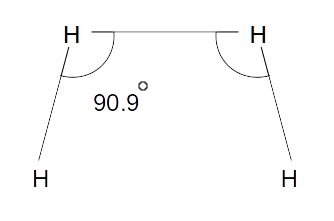
\includegraphics[width=0.4\textwidth]{h4_geo.png}
\caption{The geometry of H$_4$ used in the calculations. All bond lengths are fixed at 1.05836 \AA. Angles are in degrees.}
\label{fig:h4geo}
\end{figure}

For H$_4$, a nonstandard, minimal basis was used.\cite{h4basis} The geometry of H$_4$ was fixed to the planar geometry pictured in Figure \ref{fig:h4geo}. 13 SCF solutions were found. Three different sets of options discussed in Section \ref{sec:scfmdalg}  were utilized in order to find all 13 solutions.

\begin{table}
\centering
\begin{tabular}{c|cc} \hline\hline
Soln. Number & Lit\cite{scfmd} & This Work \\ \hline
1 & -1.8714 & -1.8714$^a$ \\
2 & -1.8513 & -1.8513$^a$ \\
3 & -1.8151 & -1.8151$^a$ \\
4 & -1.0329 & -1.0329$^a$ \\
5 & -0.8209 & -0.8209$^a$ \\
6 & -0.1485 & -0.1485$^a$ \\
7 & -0.1330 & -0.1330$^a$ \\
8 & -0.1329 & -0.1329$^a$ \\
9 & -0.1235 & -0.1235$^b$ \\
%10 & -0.1234 & -0.1234$^c$ \\
10 & -0.1171 & -0.1171$^a$ \\
11 & -0.1162 & -0.1162$^a$ \\
12 & -0.0940 & -0.0940$^a$ \\ \hline\hline
\end{tabular}
\caption{Comparison of SCF solutions found in the original SCF metadynamics publication\cite{scfmd} and this work. The parameters used to obtain these values are described below.\\
$^a$ $N_x^0 = 0.1$, $\lambda_x^0 = 1$, $s_N = 1.1$, $s_\lambda = 1.1$. New density matrix in the biased SCF loop is generated using Option C when SCF does not converge. New density matrix in the unbiased SCF loop is generated using Option D when SCF does not converge. New density matrix after convergence is generated using Option B.\\
$^b$ $N_x^0 = 0.1$, $\lambda_x^0 = 10$, $s_N = 1.1$, $s_\lambda = 1.1$. New density matrix in first SCF loop is generated using Option C. New density matrix in the second SCF loop is generated using Option D. New density matrix after convergence is generated using Option B followed by Option A.}
%$^c$ Solution calculated using the solution density matrix as the starting guess.}
\label{tab:h4results}
\end{table}

Similar to the original publication on SCF metadynamics,\cite{scfmd} this study finds the same 13 SCF solutions and these are listed in comparison to the original publication in Table \ref{tab:h4results}. From this table, it is seen that the solutions obtained within this study agree with the previous solutions to under $10^{-4}$ $E_h$. 

As these solutions are sensitive to the various SCF metadynamics parameters, and the original publication did not specify these parameters, the solutions here are obtained from two different sets of parameters. The details of these parameters are listed under Table \ref{tab:h4results}. However, one of the solutions, Solution 10, could not be found using the SCF metadynamics method, most likely due to its proximity to Solution 9. Instead, an SCF calculation using the same program was ran starting from the correct density matrix given in the original publication. From the correct density matrix, the calculation converged to the same Solution 10 in the paper. This confirms that the solution is a stationary point in the HF equations. This issue also serves as a cautionary warning. It is impossible to fully explore the space of density matrices and it is difficult to find nearly degenerate solutions. 

In terms of practical implementation, a variety of different parameters were necessary in order to obtain all solutions. Without \textit{a priori} knowledge of the number of solutions, it would be difficult to determine when all solutions have been found, of if important solutions have been missed if one set of parameters does not provide for an exhaustive search. Moreover, the SCF metadynamics algorithm would converge to these solutions within a wide range of times. Some solutions would be found in seconds, whereas others required hours of searching. The length of time required to find these solutions is also unacceptable for practical use. There is much to be desired for rigorous starting conditions and efficiency of the search in SCF metadynamics.

A stability analysis done previously concluded that only Solutions 1 and 2 are minimum, with the rest as maximums or saddle-points. An FCI calculation done in Q-Chem\cite{qchem} using the same basis finds the following as the energies (in $E_h$) of the lowest five electronic states: -1.9806, -1.8685, -1.8292, -1.4240, -1.4156. Although Solutions 1 and 2 are near true energies, the SCF results are not within chemical accuracy. Furthermore, the FCI solutions at -1.4240 and -1.4156 seem to be completely absent in the SCF solutions. It is believed that SCF solutions themselves do not accurately represent excited states for H$_4$, and further extensions are required.

\subsection{N$_2$ Results}
The dissociation of N$_2$ is a challenging problem in quantum chemistry. RHF is an appealing single reference starting point to study this system, since the RHF solutions suffer no spin-contamination unlike UHF solutions. The binding curve for N$_2$ was calculated from $r = 0.75$ \AA\ to $r = 3.20$ \AA\ in step sizes of $0.05$ \AA. The basis set used for the calculation was cc-pVDZ\cite{dunning}. All SCF solutions below -108 $E_h$ were included. The initial $N_x^0$ and $\lambda_x^0$ for each solution were 0.1 and 1 respectively. The scaling factors were set to $s_N = s_\lambda = 1.1$. Within each SCF loop, if the SCF procedure did not converge, Option C was chosen to change the density matrix (do nothing) and after the final energy is obtained, Option A (orbital rotation) was used to choose a new density matrix. DM convergence criterion was used to test for convergence and MOM was not used in either SCF loops.

\begin{figure}
\includegraphics[width=0.5\textwidth]{n2_scan.png}
\caption{The binding curves of N$_2$ calculated using RHF. These include the lowest symmetric (thick, solid, red), lowest broken-symmetry (thick, dotted, blue), another solution breaking off from the symmetric RHF solution (thin, dot-dashed, blue), and the remaining RHF solutions (thin, solid, magenta).}
\label{fig:n2plot}
\end{figure}

The binding curve for N$_2$ is plotted in Figure \ref{fig:n2plot}. The solution regarded as the RHF solution is plotted as the thick, solid, red line. The orbitals for this solution are restricted to transform with the point group of the molecule. Beyond 1.4 \AA, this solution is no longer the lowest energy, and becomes a saddle point with negative orbital Hessian eigenvalues.\cite{scfmd} Instead, lower RHF solutions result from the breaking of orbital symmetry and these are plotted in blue. The first appears at 1.4 \AA\ and the second appears at 1.7 \AA. Previous work has identified this observation as a localization of two electrons onto an orbital on each of the nitrogen atoms, leaving only one pair of electrons delocalized in a $\sigma$-bond.\cite{scfmd} Further orbital analysis needs to be conducted to draw these conclusions from this study.

\section{Conclusions and Outlook}
\label{sect:Concl}

In this study, multiple RHF solutions to H$_4$ and N$_2$ were found using an approach inspired by metadynamics. A metric was defined over the space of density matrices. A biasing potential was added to the RHF equations that allowed the SCF method to converge to a solution different from previous solutions. All of the SCF solutions to H$_4$ were found using this method and the results were compared to further FCI calculations, showing some but not completely satisfactory agreement. Finally, multiple binding curves for N$_2$ were calculated using RHF/cc-pVDZ. Besides from the RHF solution that preserves point group symmetry, other symmetry broken solutions were also found that better approximated the true binding curve.

The implementation of the SCF metadynamics method is not yet as robust as one may hope. A variety of different conditions and parameters had to be implemented and tested individually in order to obtain the solutions in this study. Moreover, many of these methods relied on random numbers, which may lead to different solutions depending on the random number generator implemented. Until more rigorous criteria are established to choose between the different implementations of SCF metadynamics discussed in Section \ref{sec:scfmdalg}, it will be difficult to apply SCF metadynamics as a black-box method for any molecule. Further work to develop a more robust implementation must be undertaken for this method to be widely applied.

It is also worth mentioning that in no previous literature regarding this method has there been mention of using MOM.\cite{scfmd,thom-2009}. From this work, it is found that MOM, in some cases, is necessary to search SCF solution space. In the case of H$_4$, MOM was necessary to obtain more than three solutions.

Another critique of this method is the large variety in convergence time for each solution. In the analysis of H$_4$, a range of times from seconds to hours were required for SCF metadynamics to converge to each solution. In practical implementations, waiting hours for a solution that may or may not exist is unacceptable. As it stands currently, SCF metadynamics requires a more efficient means to search the solution space to be feasible.

Despite the shortcomings of SCF metadynamics, SCF solutions to the RHF equations are appealing for further studies because these solutions are size-extensive. These solutions can ultimately be used as reference states for size-extensive CI calculations, short of FCI.\cite{thom-2009} The complication to CI methods using SCF solutions as a basis is that the SCF solutions disappear at certain geometries, for example at 1.40 \AA\ in the N$_2$ binding curve (Figure \ref{fig:n2plot}). Outside of these troubled points, it can be seen that the SCF solutions are retained at each geometry. This is hopeful because by recovering the lost solution at troubled points, there is a possibility that the number of SCF solutions will also be constant along the whole binding curve. Effort has been made to this end in recent work. The energy functional in the SCF method was modified to be holomorphic. This method allowed for a constant number of SCF solutions at every point on the binding curve, allowing for a CI calculation starting from the SCF solutions.\cite{thom-2014} CI using these SCF solutions have given nearly the same accuracy as FCI.\cite{thom-2016} A natural extension to this project is to find a constant number of SCF solutions across the whole binding curve using the holomorphic HF formalism.\cite{thom-2014}


\section*{Acknowledgements}
I thank my supervisor, Dr.\ Alex Thom, and the rest of my group for their guidance and patience. I would also like to thank the Sir Winston Churchill Foundation of the USA for funding.

%% The Appendices part is started with the command \appendix;
%% appendix sections are then done as normal sections




%% References
%%
%% Following citation commands can be used in the body text:
%% Usage of \cite is as follows:
%%   \cite{key}         ==>>  [#]
%%   \cite[chap. 2]{key} ==>> [#, chap. 2]
%%

%% References with bibTeX database:

\bibliographystyle{elsarticle-num}
\bibliography{references}

%% Authors are advised to submit their bibtex database files. They are
%% requested to list a bibtex style file in the manuscript if they do
%% not want to use elsarticle-num.bst.

%% References without bibTeX database:

% \begin{thebibliography}{00}

%% \bibitem must have the following form:
%%   \bibitem{key}...
%%

% \bibitem{}

% \end{thebibliography}


\end{document}

%%
%% End of file `elsarticle-template-num.tex'.
